\chapter{Hiukkassuodatin}%
\label{ch:dpf}



\begin{figure}[H]
    \centering
    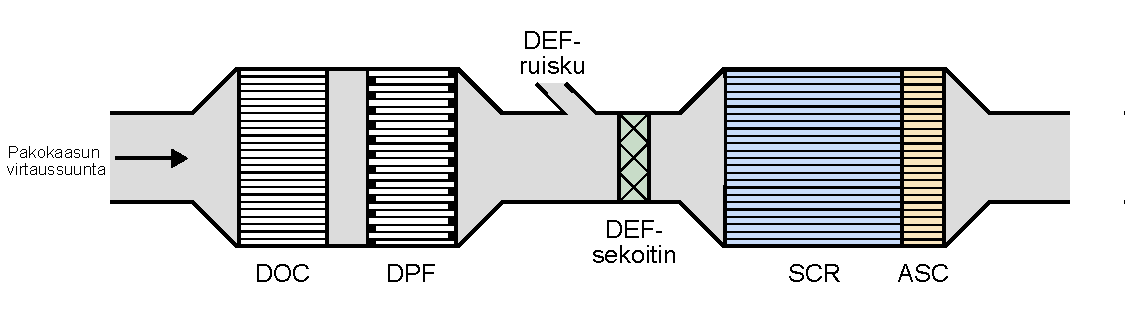
\includegraphics[width=\textwidth]{figures/EAT.pdf}
    \caption{Moderni jälkikäsittelyjä}
\end{figure}


Dieselmoottorin hiukkassuodatin, eli DPF (\emph{eng. Diesel Particulate Filter}) on tehokkain järjestelmä pakokaasun noki- ja tuhkapartikkeleiden suodatukseen. 
Hyvä DPF suodattaa läpivirtaavasta pakokaasusta jopa 99\% hiukkaslukumäärästä ja 95\% -massasta \cite{Yan_state_of_the_art}. 


\section{Järjestelmän fyysinen rakenne}

Tyypillisin DPF-tyyppi on ns. seimämävirtaus-DPF (\emph{eng. wall-flow DPF}), jossa pakokaasu virtaa vuoronperään vastakkaisista päistään suljetuissa putkissa. Pakokaasu virtaa putkien välillä huokoisten seinämien läpi. Virtausta on havainnollistettu Kuvassa \ref{fig:wall-flow-dpf}  


\begin{figure}[H]
    \centering 
    
    \pdftooltip{
\begin{tikzpicture}[scale=2]
    % Drawing gray squares between the lines
    \fill[gray] (0, 0) rectangle (0.5, 0.5);  
    \fill[gray] (0, 1.0) rectangle (0.5, 1.5); 
    \fill[gray] (4.5, 0.5) rectangle (5, 1.0); 
    \fill[gray] (4.5, 1.5) rectangle (5, 2.0); 
    
    % Drawing 5 parallel horizontal lines with 0.5 unit spacing
    \foreach \y in {0, 0.5, 1, 1.5, 2} {
        \draw[line width=3pt, black]  (0, \y) -- (5, \y);
    }
    % For widening the lines
    % \draw[line width=3pt, black]  (0, -0.05) -- (5, -0.05);
    % \draw[line width=3pt, black]  (0, 2.05) -- (5, 2.05);

    % Adding arrows pointing to the gaps with no squares
    \draw[-{Latex}, thick, red] (-1, 0.75) -- (-0.1, 0.75);
    \draw[-{Latex}, thick, red] (-1, 1.75) -- (-0.1, 1.75); 
    \draw[-{Latex}, thick, red] (5.1, 0.25) -- (6, 0.25); 
    \draw[-{Latex}, thick, red] (5, 1.25) -- (6, 1.25); 

   \draw[-{Latex}, thick, red] (0.5, 0.75) to[out=0, in=180] (1.5, 0.25);
    \draw[-{Latex}, thick, red] (0.5, 0.75) to[out=0, in=180] (1.5, 1.25);
    \draw[-{Latex}, thick, red] (2.5, 0.75) to[out=0, in=180] (3.5, 0.25);
    \draw[-{Latex}, thick, red] (2.5, 0.75) to[out=0, in=180] (3.5, 1.25);
    
    
    
    \draw[-{Latex}, thick, red] (1.5, 1.75) to[out=0, in=180] (2.5, 1.25);
    \draw[-{Latex}, thick, red] (3.5, 1.75) to[out=0, in=180] (4.5, 1.25);
\end{tikzpicture}

}
                {Kuvituskuvassa on neljä päällekkäistä putkea. Nuolilla kuvattu pakokaasu virtaa vasemmalta avoimiin putkiin. Putket ovat suljettuja oikeasta päästään, joten nuolet kulkevat putkien välisen seinämän läpi putkiin, jotka ovat avoimia oikealta. Nuolet poistuvat putkista oikealta puolelta.
                }
    \caption{Pakokaasu virtaa suodattimessa huokoisten seinämien läpi. Yli 90\% pakokaasun hiukkasmassasta jää huokoisten seinämien sisään ja pinnalle.}
    \label{fig:wall-flow-dpf}
\end{figure}



\section{Regenerointi}
\begin{align*}
    \ce{C + 1/2 O2 &-> CO }\\
    \ce{C + O2 &-> CO2}\\
    \ce{C + NO2 &-> CO +  NO}  \\
    \ce{C + 2 NO2 &-> CO2 + 2 NO}  \\
    \ce{C + NO2 + 1/2 O2 &-> CO2 + NO}  \\
    \ce{C + NO2 + 1/2 O2 &-> CO + NO2} 
\end{align*}


\section{Hiukkassuodattimen matemaattinen esitys}

\begin{figure}[H]
    \centering 
    \begin{tikzpicture}
    % Draw the first rectangle
    \node[draw, rectangle, minimum width=1.5cm, minimum height=3cm] (rect1) at (0, 0) {Rectangle 1};

    % Draw the second rectangle
    \node[draw, rectangle, minimum width=1.5cm, minimum height=3cm] (rect2) at (4, 0) {Rectangle 2};

    % Draw arrows between rectangles
    \draw[-{Latex}, thick] ([yshift=-0.5cm]rect1.north east) -- ([yshift=-0.5cm]rect2.north west);
    \draw[-{Latex}, thick] ([yshift=0.5cm]rect1.south east) -- ([yshift=0.5cm]rect2.south west);

    % Draw inputs to rect1
    \draw[-{Latex}, thick] (-3, 1) -- ([yshift=1cm]rect1.west) node[above left] {Nokilataus (g/l)};
    \draw[-{Latex}, thick] (-3, -1) -- ([yshift=-1cm]rect1.west) node[below left] {Tuhkalataus (g/l)};

    % Draw output from rect2
    \draw[-{Latex}, thick] (rect2.east) -- (7, 0) node[above right] {Paine (hPa)};

\end{tikzpicture}
    \caption{}
    \label{fig:blocks1}
\end{figure}
\cite{LiuGuanlin2021Roio}
